\documentclass{article}
\usepackage[utf8]{inputenc}
\usepackage{geometry}
\usepackage{graphicx}
\usepackage{amsmath}
\usepackage{amsfonts}
\usepackage{amsthm}
\usepackage{amssymb}
\usepackage[most]{tcolorbox}
\usepackage{array}
\usepackage{latexsym}
\usepackage{alltt}
\usepackage{hyperref}
\usepackage{color, colortbl}
\usepackage{float}
\usepackage{pdfpages}
\usepackage{algpseudocode}
\usepackage{multicol}
\usepackage{multirow}
\usepackage{caption}
\usepackage{xparse}
\usepackage{setspace}
\usepackage{enumitem}
\usepackage{pdflscape}
% \usepackage{parskip}
\usepackage{blindtext}
\usepackage{forest}
% \usepackage[newfloat]{minted}
\usepackage{booktabs}


\geometry
{
  a4paper,
  left=12mm,
  right=12mm,
  top=12mm,
  bottom=15mm,
}

% mybox
\newtcolorbox{mybox}[3][]
{
  colframe = #2!25,
  colback  = #2!10,
  coltitle = #2!20!black,  
  title    = {#3},
  #1,
}

\definecolor{ex}{rgb}{1.00,0.65,0.00}
\definecolor{bg}{rgb}{0.95,0.95,0.95}
% \setminted
% {
% 	mathescape=true,
% 	xleftmargin=\parindent,
% 	bgcolor=bg,
% 	escapeinside=@@
% }

% \SetupFloatingEnvironment{listing}{name=Code}

% New environments that use mybox
\newcounter{example}[section]
\newenvironment{example}[1]{\begin{mybox}[breakable]{ex}{\refstepcounter{example}\textbf{Example \thesection.\theexample #1}}}{\end{mybox}}

\newcounter{definition}[section]
\newenvironment{definition}[1]{\refstepcounter{definition}\begin{mybox}[breakable]{blue}{\textbf{Definition \thesection.\thedefinition #1}}}{\end{mybox}}

\newcounter{theorem}[section]
\newenvironment{theorem}[1]{\begin{mybox}{red}{\refstepcounter{theorem}\textbf{Theorem \thesection.\thetheorem #1}}}{\end{mybox}}

\newenvironment{formula}[1]{\begin{mybox}{cyan}{\textbf{#1}}}{\end{mybox}}

\newenvironment{practice}[1]{\begin{mybox}{ex}{\textbf{#1}}}{\end{mybox}}

% Changing maketitle
\makeatletter         
\renewcommand\maketitle{
{\raggedright % Note the extra {
\begin{center}
{\Large \bfseries \@title}\\[2ex] 
{\large \@author \ - \@date}\\[2ex]
\end{center}}} % Note the extra }
\makeatother

% \onehalfspacing % adjust spacing
\setlength{\parskip}{0.5\baselineskip}

% macros
\newcommand{\prob}[1]{\textbf{\textit{P}}\left\{#1\right\}}
\newcommand{\expc}[1]{\mathbf{E}\left(#1\right)}
\newcommand{\expcs}[1]{\mathbf{E}^2\left(#1\right)}
\newcommand{\var}[1]{\text{Var}\left( #1 \right)}
\newcommand{\ra}{\rightarrow}
\newcommand{\Ra}{\Rightarrow}
\newcommand{\R}[2]{\tikz [remember picture,overlay] \node (#1) {#2};}

\def\circtxt#1{$\mathalpha \bigcirc \mkern-13mu \mathtt #1$}
\def\smiley{\textcircled{\scriptsize $\mkern3mu\ddot{\ } \mkern-15mu \smallsmile$}}

\NewDocumentCommand{\dsum}{%
    e{^_}
}{%
  {% 
    \displaystyle\sum
    \IfValueT{#1}{^{#1}}
    \IfValueT{#2}{_{#2}}
  }
}%

% maketitle variables
\title{CENG 232 - Chapter 5: Synchronous Sequential Logic}
\author{Burak Metehan Tunçel}
\date{May 2022}

\begin{document}

\maketitle

\begin{multicols*}{2}
\setlength{\columnsep}{1.5cm}
\setlength{\columnseprule}{0.2pt}

\section{Sequential Circuits}
\label{sec:seq-cir}

Figure 5.1 shows a block diagram of a sequential circuit. It consists of a combinational circuit to which memory elements are connected to form a feedback path. The storage elements are devices capable of storing binary information. The binary information stored in these elements at any given time defines the state of the sequential circuit at that time.

\begin{figure}[H]
  \centering
  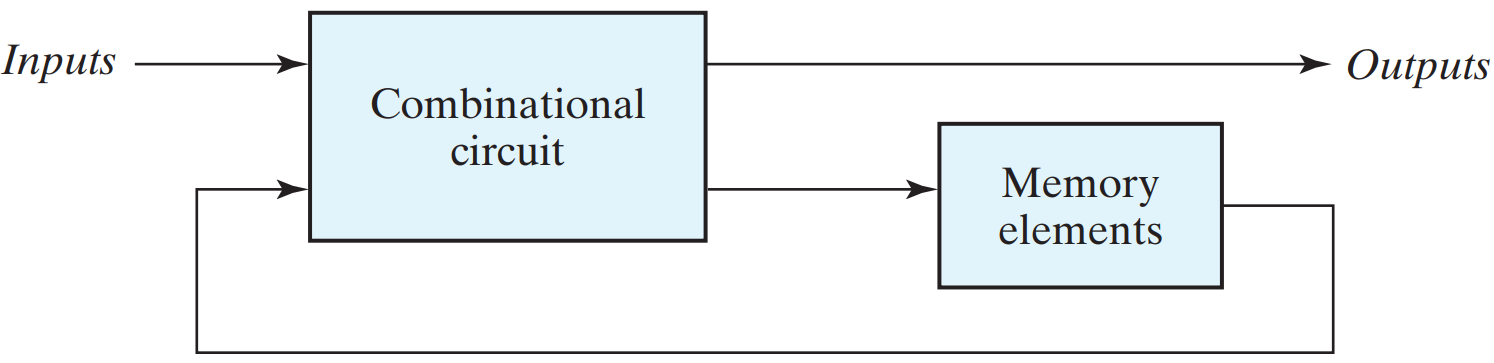
\includegraphics[width=\linewidth]{img/fig-5.1.png}
  \caption{Block diagram of sequential circuit}
  \label{fig:5.1}
\end{figure}

The block diagram demonstrates that the outputs in a sequential circuit are a function not only of the inputs but also of the present state of the storage elements. The next state of the storage elements is also a function of external inputs and the present state. Thus, \textit{\textbf{a sequential circuit is specified by a time sequence of inputs, outputs, and internal states}}.

There are two main types of sequential circuits, and their classification is a function of the timing of their signals:
\begin{itemize}
  \item A \textit{\textbf{synchronous} sequential circuit} is a system whose behavior can be defined from the knowledge of its signals at discrete instants of time.
  \item The behavior of an \textit{\textbf{asynchronous} sequential circuit} depends upon the input signals at any instant of  time \textit{and} the order in which the inputs change
\end{itemize}

A synchronous sequential circuit employs signals that affect the storage elements at only \textit{discrete instants of time}. Synchronization is achieved by a timing device called a \textit{clock generator}, which provides a clock signal having the form of a periodic sequence of clock pulses. In practice, the clock pulses determine when computational activity will occur within the circuit, and other signals (external inputs and otherwise) determine what changes will take place affecting the storage elements and the outputs.

Synchronous sequential circuits that use clock pulses to control storage elements are called \textit{clocked sequential circuits} and are the most 
frequently encountered type in practice. They are called \textit{synchronous circuits} because the activity within the circuit and the resulting updating of stored values is synchronized to the occurrence of clock pulses.

The storage elements (memory) used in clocked sequential circuits are called \textit{flip-flops}. A flip-flop is a binary storage device capable of storing one bit of information. In a stable state, the output of a flip-flop is either 0 or 1.

The block diagram of a synchronous clocked sequential circuit is shown in  Fig. 2. 
\begin{figure}[H]
  \centering
  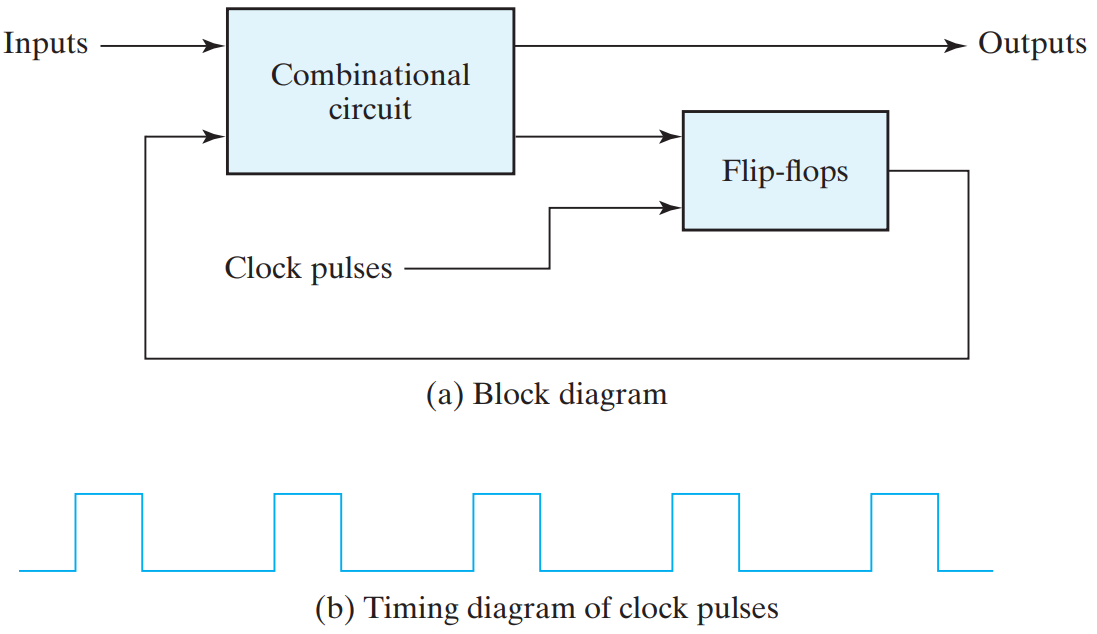
\includegraphics[width=\linewidth]{img/fig-5.2.png}
  \caption{Synchronous clocked sequential circuit}
  \label{fig:5.2}
\end{figure}

\begin{itemize}
  \item The \textit{outputs} are formed by a \textit{combinational logic function of the inputs to the circuit or the values stored in the flip-flops (or both)}. 
  \item The \textit{value that is stored in a flip-flop} when the clock pulse occurs is also determined by \textit{the inputs to the circuit or the values presently stored in the flip-flop (or both)}.
  \item The \textit{new value is stored} (i.e., the flip-flop is \textit{updated}) when a pulse of the clock signal occurs. Prior to the occurrence of the clock pulse, the combinational logic forming the next value of the flip-flop must have reached a stable value.
\end{itemize}

\begin{practice}{Practice Exercise 5.1}
Describe the fundamental difference between the output of a combinational circuit and the output of a sequential circuit. \\

\textbf{Answer:} 
The output of a combinational circuit depends on only the inputs to the circuit; the output of a sequential circuit depends on the inputs to the circuit and the present state of the storage elements.
\end{practice}


\section{Storage Element: Latches}
\label{sec:stor-ele-latch}

A storage element in a digital circuit can maintain a binary state indefinitely (as long as power is delivered to the circuit), until directed by an input signal to switch states.

\textit{Storage elements that operate with signal levels (rather than signal transitions) are referred to as latches; those controlled by a clock transition are flip-flops}.

Latches are said to be \textit{level-sensitive devices}; flip-flops are \textit{edge-sensitive devices}. The two types of storage elements are related because \textit{latches are the basic circuits from which all flip-flops are constructed}. Although latches are useful for storing binary information and for the design of asynchronous sequential circuits, they are not practical for use as storage elements in synchronous sequential circuits.

\subsection{SR Latch}
\label{subsec:sr-latch}

The \textit{SR} latch is a circuit with two cross-coupled NOR gates or two cross-coupled NAND gates, and two inputs labeled \textit{S} for set, and \textit{R} for reset. The \textit{SR} latch constructed with two cross-coupled NOR gates is shown in Fig. 3. 
\begin{figure}[H]
  \centering
  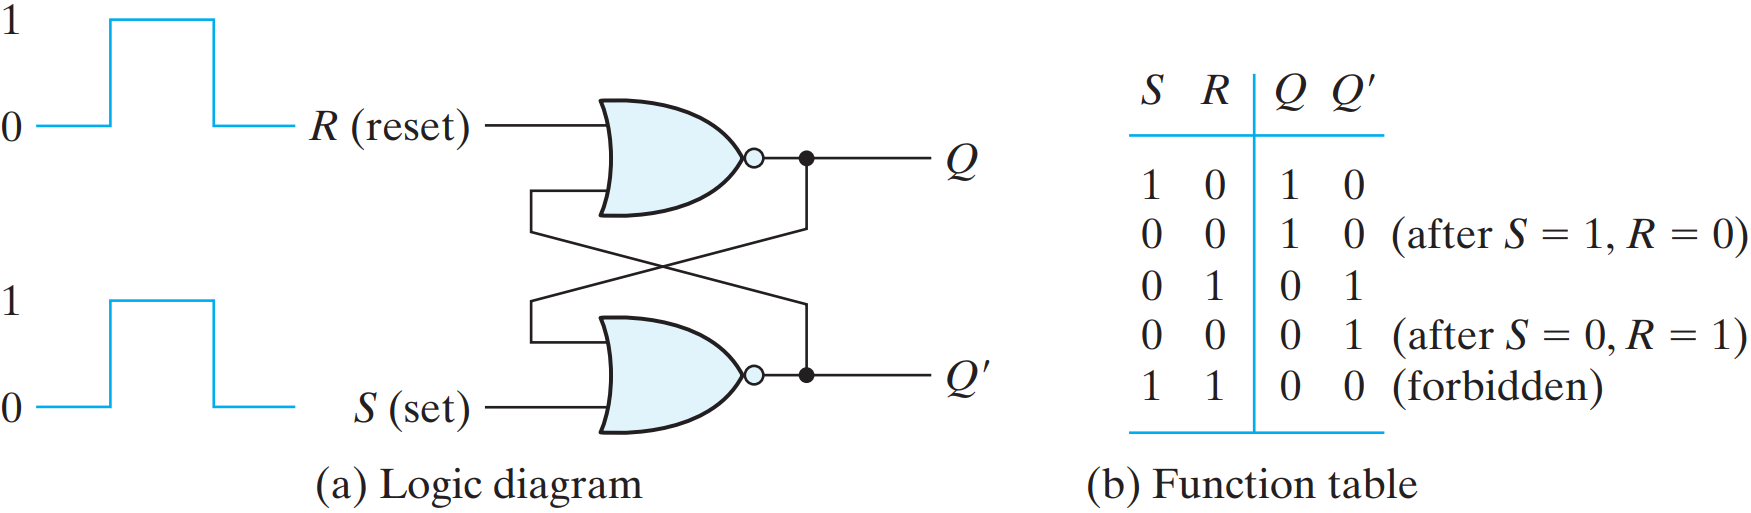
\includegraphics[width=\linewidth]{img/fig-5.3.png}
  \caption{SR latch with NOR gate}
  \label{fig:5.3}
\end{figure}
\noindent The latch has two useful states. When output $Q = 1$ and $Q' = 0$, the latch is said to be in the \textit{set} state. When $Q = 0$ and $Q' = 1$, it is in the \textit{reset} state.

However, when both inputs are equal to 1 at the same time, a condition in which both outputs are equal to 0 (rather than be mutually complementary) occurs. If both inputs are then switched to 0 simultaneously, the device will enter an unpredictable or undefined state or a metastable state. Consequently, in practical applications, \textbf{setting both inputs to 1 is forbidden}. Under normal conditions, both inputs of the latch remain at 0 unless the state has to be changed.

The \textit{SR} latch with two cross-coupled NAND gates is shown in Fig. 4. 
\begin{figure}[H]
  \centering
  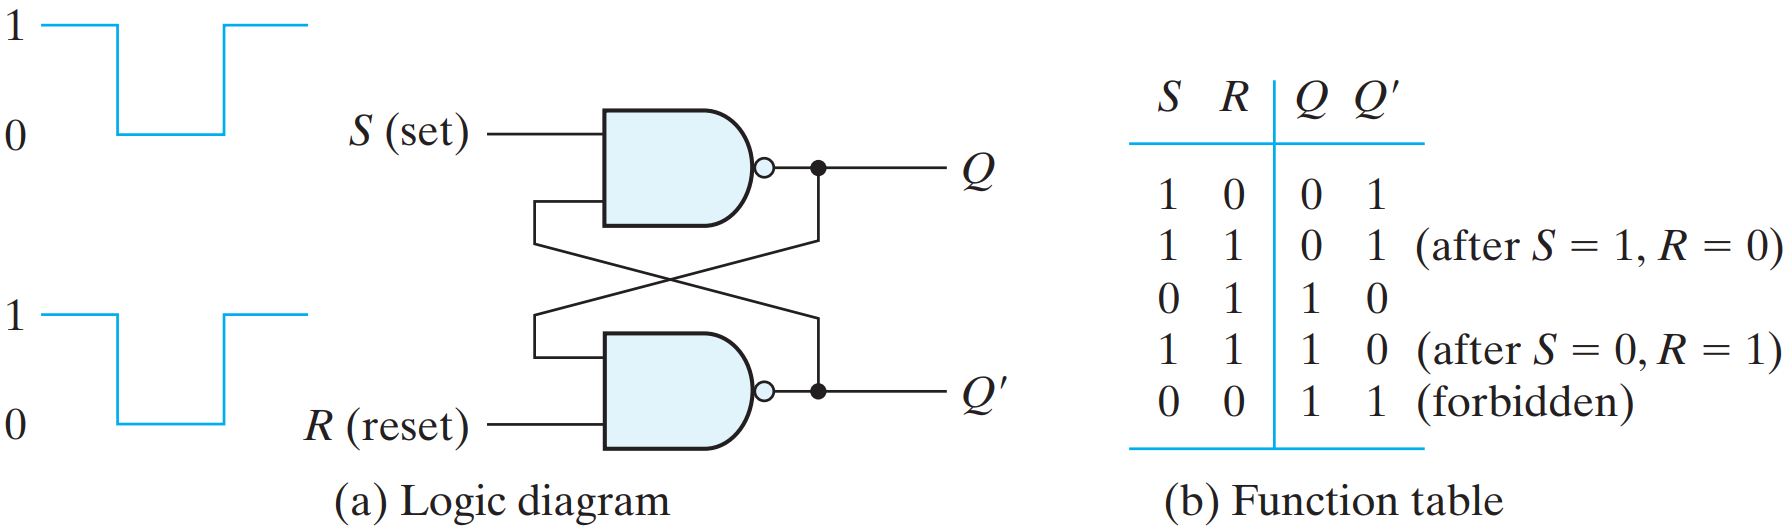
\includegraphics[width=\linewidth]{img/fig-5.4.png}
  \caption{SR latch with NAND gates}
  \label{fig:5.4}
\end{figure}
It operates with both inputs normally at 1, unless the state of the latch has to be changed. The condition that is forbidden for the NAND latch is both inputs being equal to 0 at the same time, an input combination that should be avoided.

In comparing the NAND with the NOR latch, note that the input signals for the NAND require the complement of those values used for the NOR latch. Because the NAND latch requires a 0 signal to change its state, it is sometimes referred to as an $S'R'$ latch. The primes (or, sometimes, bars over the letters) designate the fact that the inputs must be in their complement form to activate the circuit.

The operation of the basic $SR$ latch can be modified by providing an additional input signal that determines (controls) when the state of the latch can be changed by determining whether $S$ and $R$ (or $S'$ and $R'$) can affect the circuit. An SR latch with a control input is shown in Fig. 5. It consists of the basic SR latch and two additional NAND gates.
\begin{figure}[H]
  \centering
  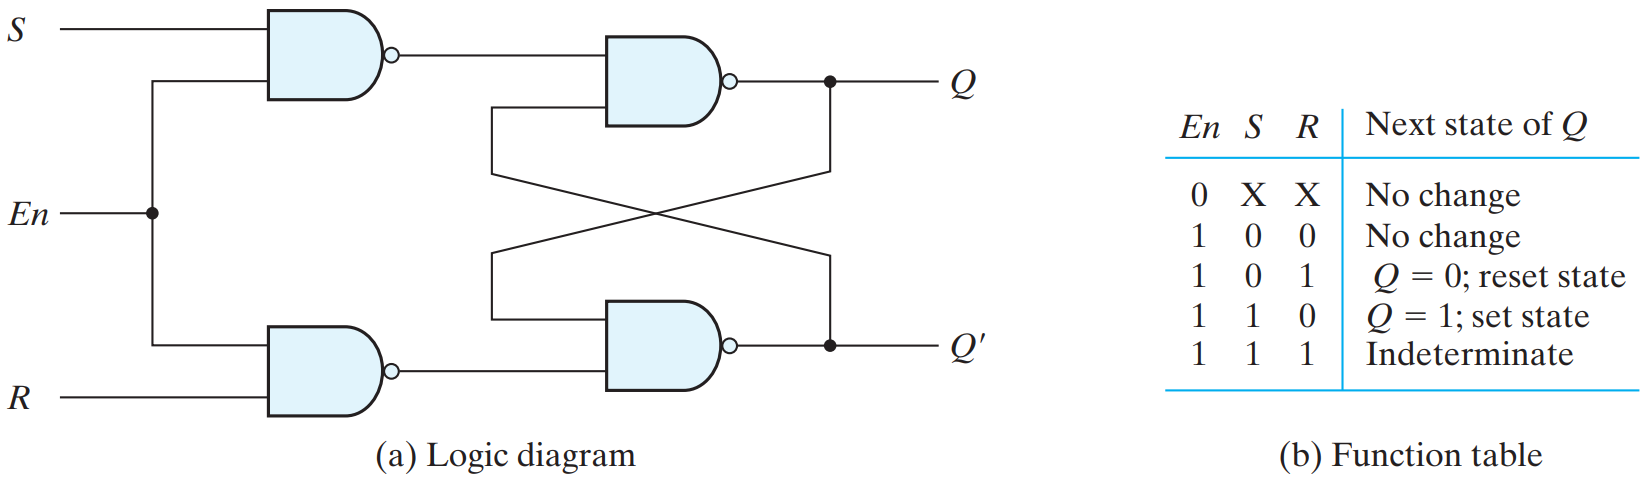
\includegraphics[width=\linewidth]{img/fig-5.5.png}
  \caption{SR latch with control input}
  \label{fig:5.5}
\end{figure}
An indeterminate condition occurs when all three inputs are equal to 1. This condition places 0's on both inputs of the basic $SR$ latch, which puts it in the undefined state.

\begin{practice}{Practice Exercise 5.2}
\begin{enumerate}[label=(\alph*), leftmargin=0.5cm]
  \item What input condition puts an $SR$ NOR latch into an indeterminate state?
  
  \textbf{Answer:} Both inputs are 1.
  
  \item What input condition puts an $SR$ NAND latch into an indeterminate state?
  
  \textbf{Answer:} Both inputs are 0.
\end{enumerate}
\end{practice}


\subsection{D Latch (Transparent Latch)}
\label{subsec:d-latch}

One way to eliminate the undesirable condition of the indeterminate state in the $SR$ latch is to ensure that inputs $S$ and $R$ are never equal to 1 at the same time. This is done in the $D$ latch, shown in Fig. 6. 
\begin{figure}[H]
  \centering
  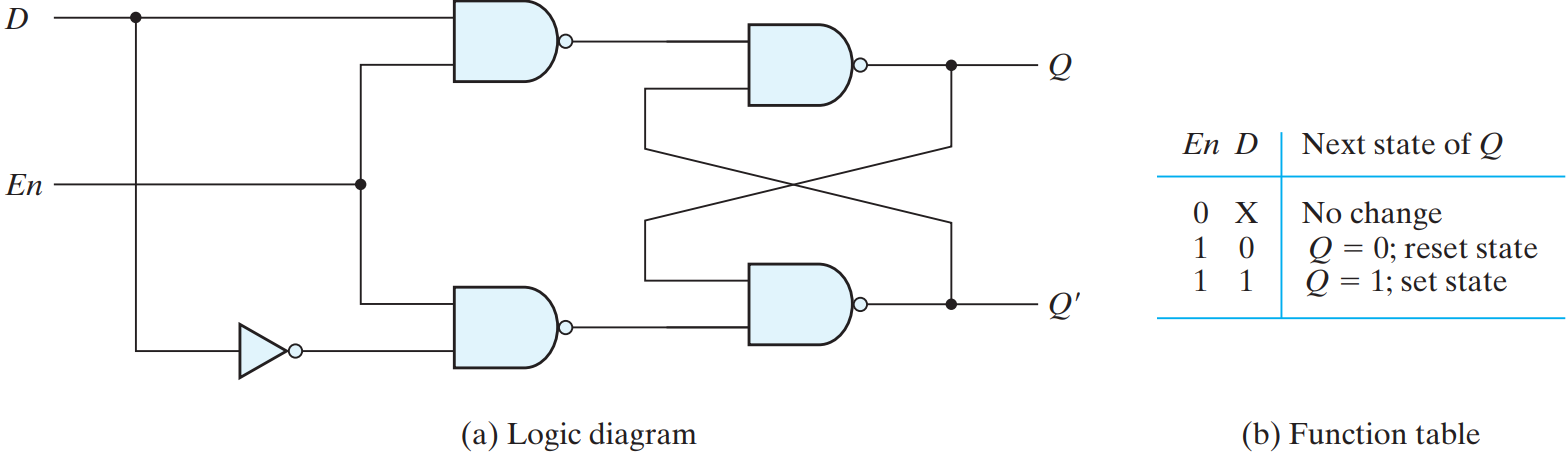
\includegraphics[width=\linewidth]{img/fig-5.6.png}
  \caption{D Latch}
  \label{fig:5.6}
\end{figure}
\noindent This latch has only two inputs: $D$ (data) and $En$ (enable). The $D$ input goes directly to the $S$ input, and its complement is applied to the $R$ input. 

The $D$ latch receives that designation from its ability to hold data in its internal storage. It is suited for use as a temporary storage for binary information between a unit and its environment. The binary information present at the data input of the $D$ latch is transferred to the $Q$ output when the enable input is asserted. The output follows changes in the data input as long as the enable input is asserted.

The circuit is often called a transparent latch. When the enable input signal is de-asserted, the binary information that was present at the data input at the time the transition of enable occurred is retained (i.e., stored) at the $Q$ output until the enable input is asserted again.

The graphic symbols for the various latches are shown in Fig. 7.
\begin{figure}[H]
  \centering
  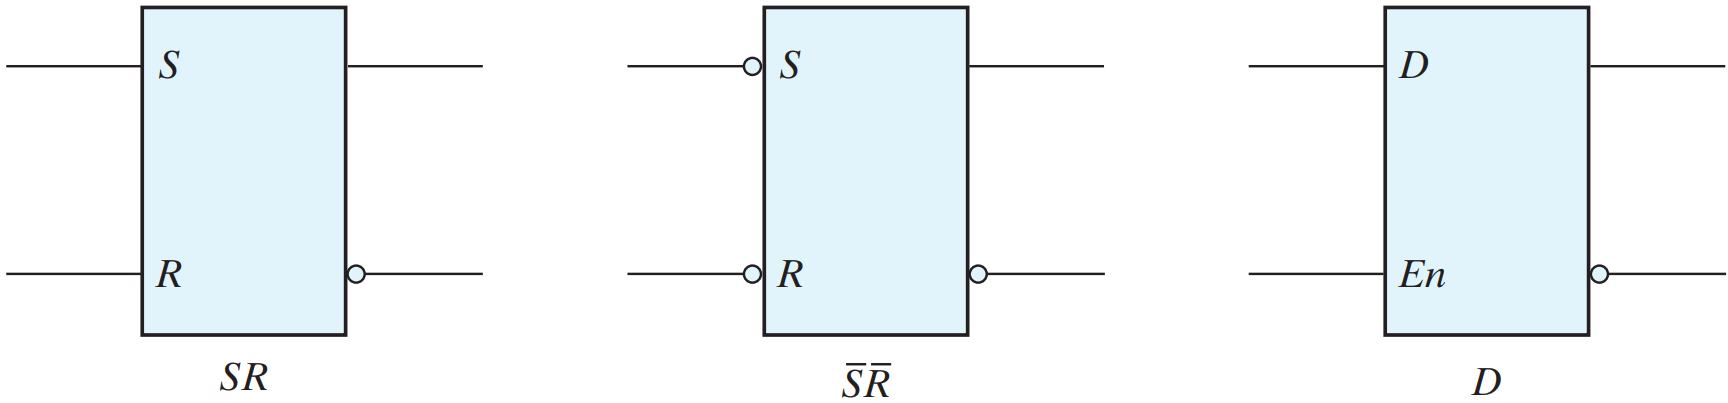
\includegraphics[width=\linewidth]{img/fig-5.7.png}
  \caption{Graphic symbols for latches}
  \label{fig:5.7}
\end{figure}

\begin{practice}{Practice Exercise 5.3}
Describe the functionality of a transparent latch. \\

\textbf{Answer:}
A transparent latch has a data input, an enable input, and output. When the enable input is asserted, the output of the latch follows the input to the latch. When the enable input is de-asserted, the output of the latch is held at the value that was present at the moment the enable input was de-asserted.
\end{practice}



\section{Storage Element: Flip-Flops}
\label{sec:stor-ele-flip-flop}

A change in the control input of a latch or flip-flop switches its state. This momentary change is called a \textit{trigger}, and the transition it causes is said to trigger the flip-flop. The $D$ latch with pulses in its control input is essentially a flip-flop that is triggered every time the pulse goes to the logic-1 level.

Flip-flop circuits are constructed in such a way as to make them operate properly when they are part of a sequential circuit that employs a common clock. The problem with the latch is that it responds to a change in the \textit{level} of a clock pulse. The key to the proper operation of a flip-flop is to trigger it only during a signal \textit{transition}.

\begin{figure}[H]
  \centering
  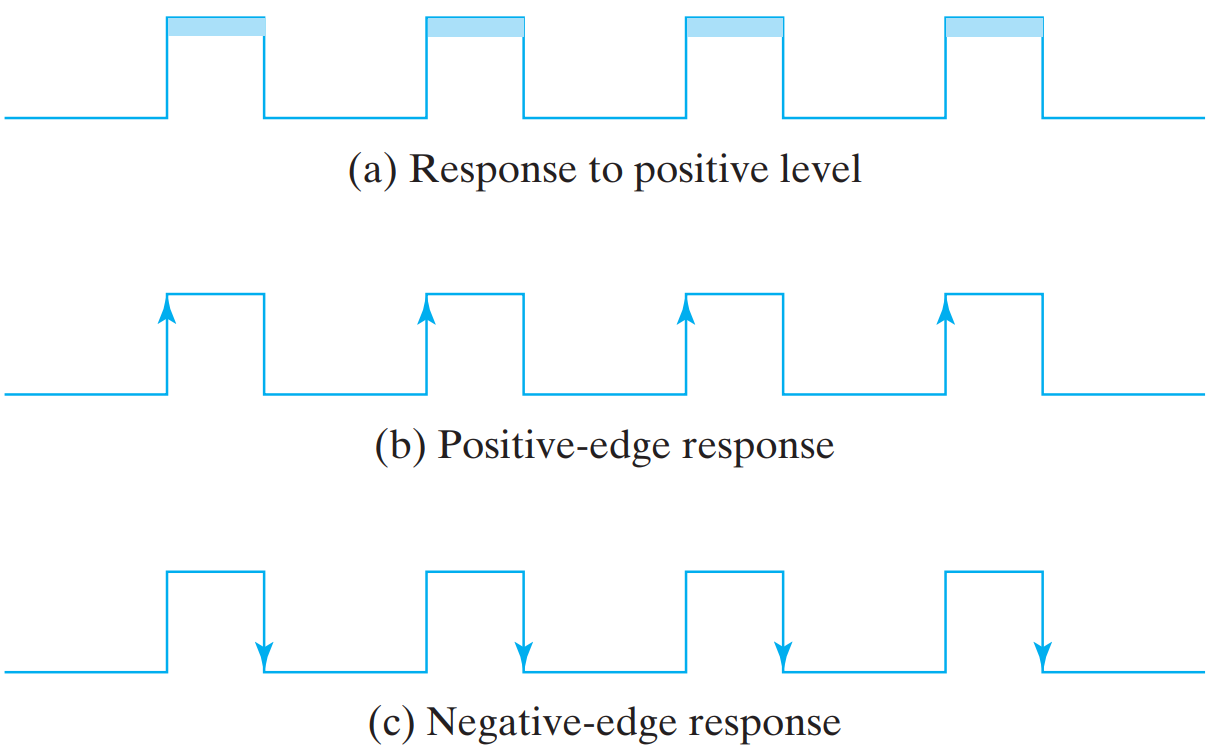
\includegraphics[width=\linewidth]{img/fig-5.8.png}
  \caption{Clock response in latch and flip-flop}
  \label{fig:5.8}
\end{figure}

There are two ways that a latch can be modified to form a flip-flop.
\begin{itemize}
  \item One way is to employ two latches in a special configuration that isolates the output of the flip-flop and prevents it from being affected while the input to the flip-flop is changing.
  \item Another way is to produce a flip-flop that triggers only during a signal transition (from 0 to 1 or from 1 to 0) of the synchronizing signal (clock) and is disabled during the rest of the clock pulse.
\end{itemize}

\subsection{Edge-Triggered D Flip-Flop}
\label{subsec:edge-trig-d-flip-flop}

The construction of a $D$ flip-flop with two $D$ latches and an inverter is shown in Fig. 9. It is often referred to as a master–slave flip-flop. The first latch is called the master and the second the slave. The circuit samples the $D$ input and changes its output $Q$ \textit{only at the negative edge} of the synchronizing or controlling clock.
\begin{figure}[H]
  \centering
  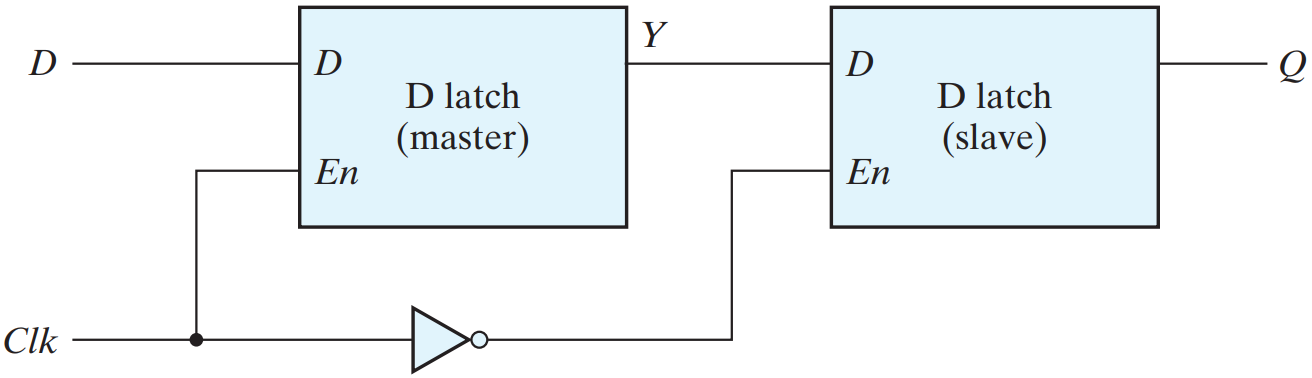
\includegraphics[width=\linewidth]{img/fig-5.9.png}
  \caption{Master–slave $D$ flip-flop}
  \label{fig:5.9}
\end{figure}
\noindent \textit{A change in the output of the flip-flop can be triggered only by and during the transition of the clock from 1 to 0}.

The behavior of the master–slave flip-flop just described dictates that
\begin{enumerate}[leftmargin=0.5cm]
  \item The output may change only once,
  \item A change in the output is triggered by the negative edge of the clock,
  \item The change may occur only during the clock's negative level.
\end{enumerate}
\noindent The value that is produced at the output of the flip-flop is the value that was stored in the master stage immediately before the negative edge occurred. It is also possible to design the circuit so that the flip-flop output changes on the positive edge of the clock.

Another construction of an edge-triggered $D$ flip-flop uses three $SR$ latches as shown in Fig. 10.
\begin{figure}[H]
  \centering
  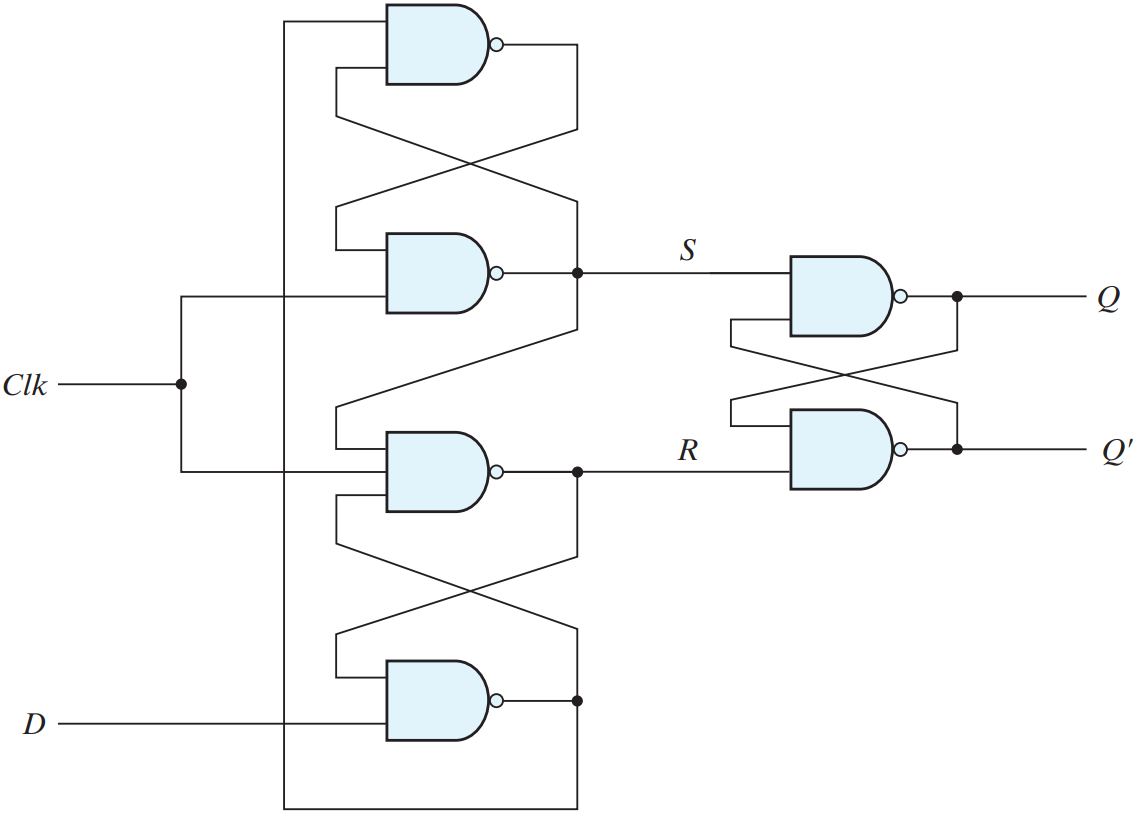
\includegraphics[width=\linewidth]{img/fig-5.10.png}
  \caption{D-type positive-edge-triggered flip-flop}
  \label{fig:5.10}
\end{figure}

In sum, \textit{when the input clock in the positive-edge-triggered flip-flop makes a positive transition, the value of \textnormal{D} is transferred to \textnormal{Q}}. A negative transition of the clock (i.e., from 1 to 0) does not affect the output, nor is the output affected by changes in $D$ when \textit{Clk} is in the steady logic-1 level or the logic-0 level.

The timing of the response of a flip-flop to input data and to the clock must be taken into consideration when one is using edge-triggered flip-flops. There is a minimum time called the setup time during which the $D$ input must be maintained at a constant value prior to the occurrence of the clock transition. Similarly, there is a minimum time called the hold time during which the $D$ input must not change after the application of the positive transition of the clock.

The graphic symbol for the edge-triggered $D$ flip-flop is shown in Fig. 11. It is similar to the symbol used for the $D$ latch, except for the arrowhead-like symbol in front of the letter \textit{Clk}, designating a \textit{dynamic} input. \textit{The dynamic indicator ($>$) denotes the fact that the flip-flop responds to the edge transition of the clock}.
\begin{figure}[H]
  \centering
  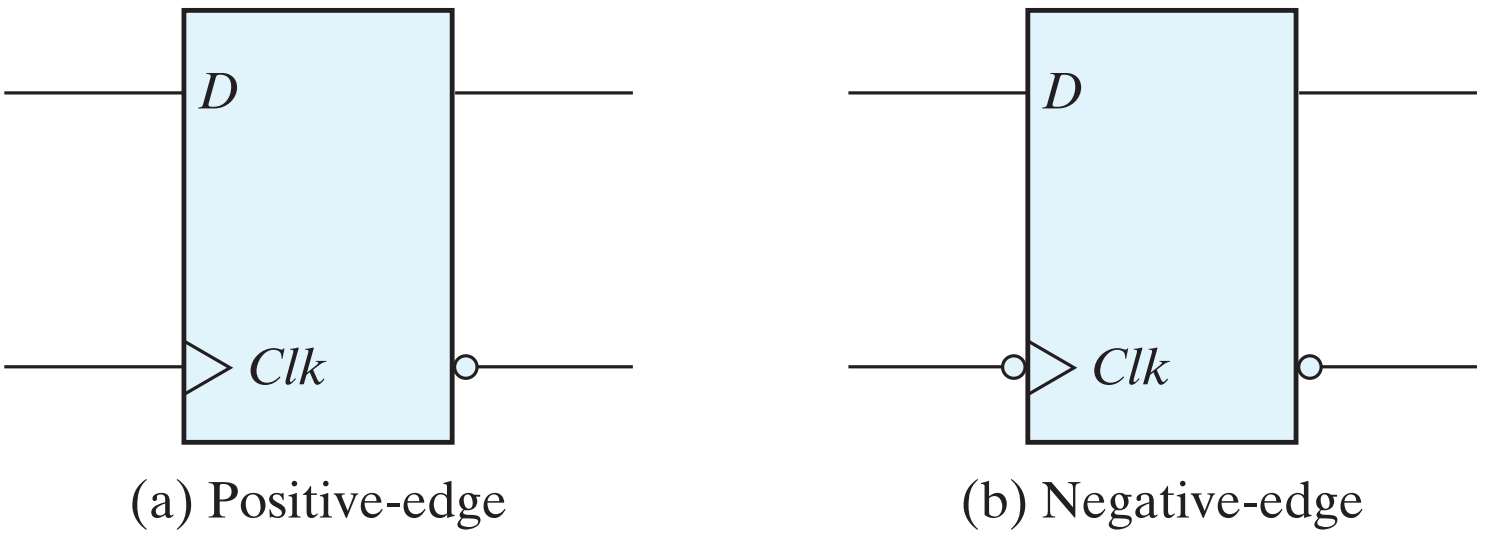
\includegraphics[width=\linewidth]{img/fig-5.11.png}
  \caption{Graphic symbol for edge-triggered D flip-flop}
  \label{fig:5.11}
\end{figure}

\begin{practice}{Practice Exercise 5.4}
\noindent What is meant by ``a positive-edge flip-flop''?\\

\textbf{Answer:} A positive-edge flip-flop is one that is activated by the rising (positive) edge of the clock (synchronizing signal).
\end{practice}

\subsection{Other Flip-Flops}
\label{subsec:other-flip-flops}

The most economical and efficient flip-flop constructed in this manner is the edge-triggered $D$ flip-flop, because it requires the smallest number of gates. Other types of flip-flops can be constructed by using the $D$ flip-flop and external logic. Two flip-flops less widely used in the design of digital systems are the $JK$ and $T$ flip-flops.

There are three operations that can be performed with a flip-flop:
\begin{enumerate}[]
  \item Set it to 1,
  \item Reset it to 0, or 
  \item Complement its output.
\noindent \end{enumerate}

\subsubsection{JK Flip-Flops}
\label{subsubsec:jk-flip-flops}

With only a single input, the $D$ flip-flop can set or reset the output. The $JK$ flip-flop has two inputs and performs all three operations. The circuit diagram of a $JK$ flip-flop constructed with a $D$ flip-flop 
and gates is shown in Fig. 12(a).
\begin{figure}[H]
  \centering
  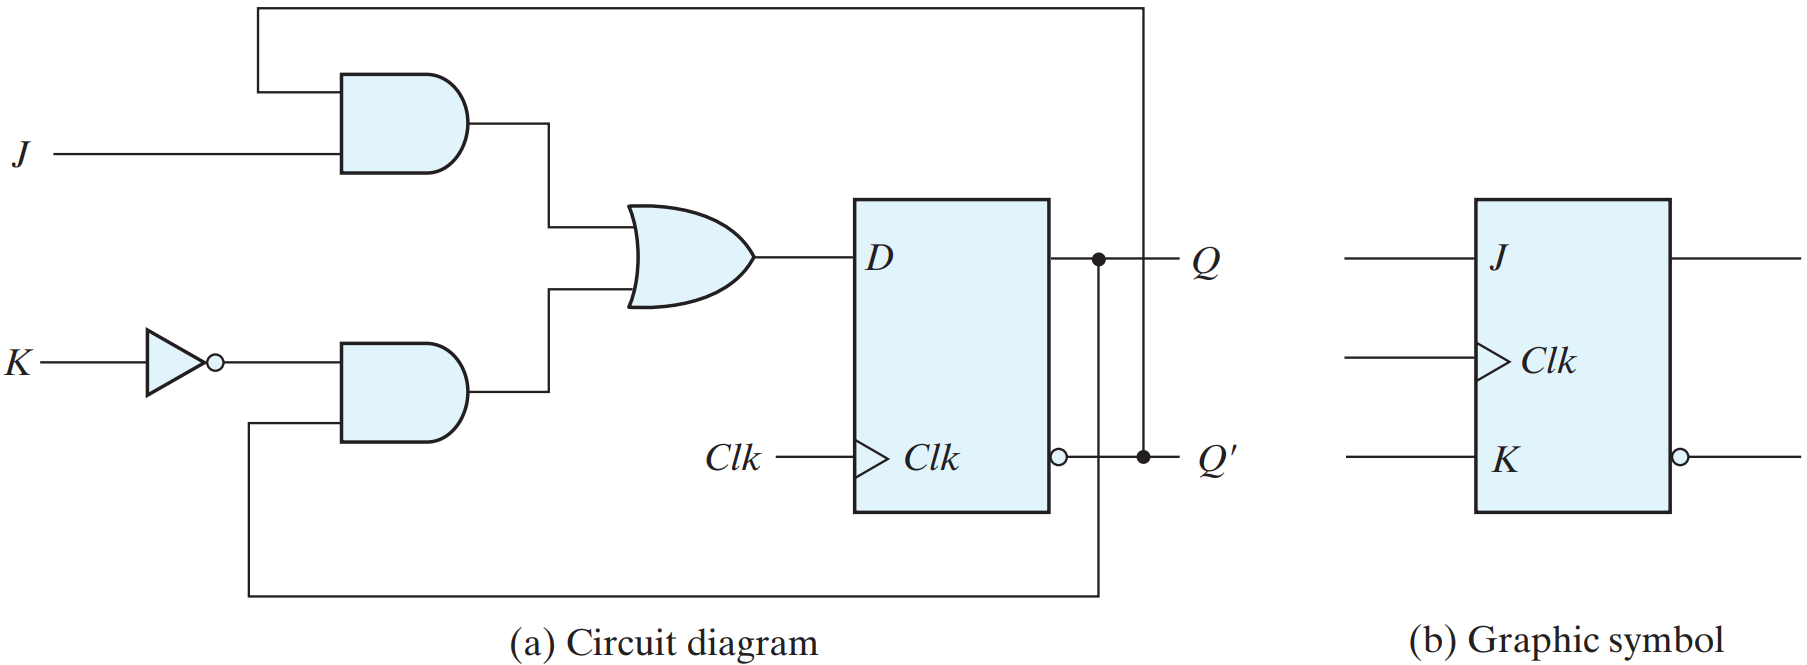
\includegraphics[width=\linewidth]{img/fig-5.12.png}
  \caption{$JK$ flip-flop}
  \label{fig:5.12}
\end{figure}
\noindent The $J$ input sets the flip-flop to 1, the $K$ input resets it 
to 0, and when both inputs are enabled, the output is complemented. This can be verified by investigating the circuit applied to the D input:
\begin{equation*}
  D = JQ' + K'Q
\end{equation*}
The graphic symbol for the $JK$ flip-flop is shown in Fig. 12(b).

\subsubsection{T Flip-Flops}
\label{subsubsec:t-flip-flops}

The $T$ (toggle) flip-flop is a complementing flip-flop and can be obtained from a $JK$ flip-flop when inputs $J$ and $K$ are tied together. This is shown in Fig. 13(a).
\begin{figure}[H]
  \centering
  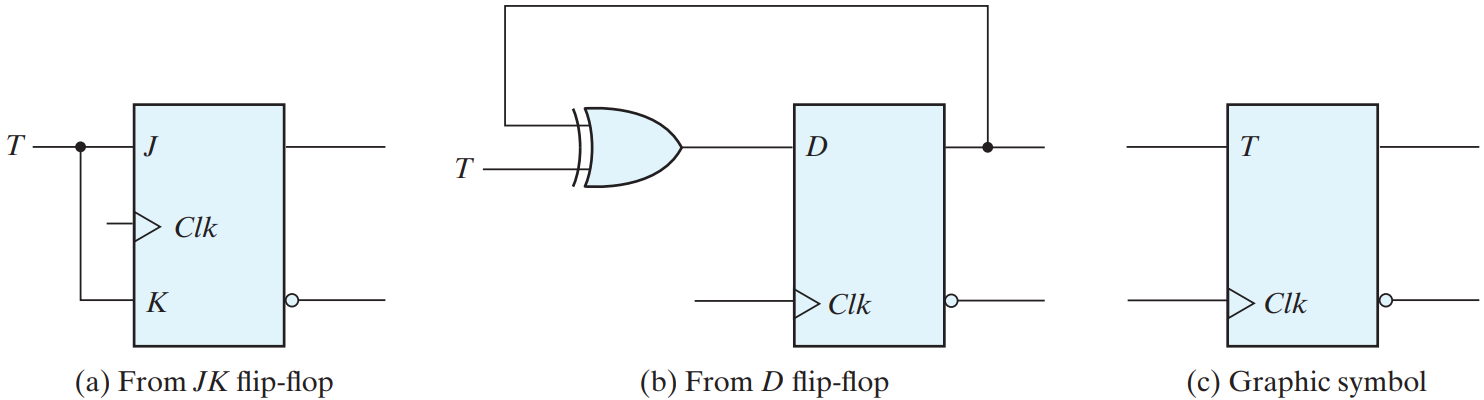
\includegraphics[width=\linewidth]{img/fig-5.13.png}
  \caption{T flip-flop}
  \label{fig:5.13}
\end{figure}
The complementing flip-flop is useful for designing binary counters. The $T$ flip-flop can be constructed with a $D$ flip-flop and an exclusive-OR gate as shown in Fig. 13(b). The expression for the D input is
\begin{equation*}
  D = T \oplus Q = TQ' + T'Q
\end{equation*}
The graphic symbol for this flip-flop has a $T$ symbol in the input.


\subsection{Characteristic Tables}
\label{subsec:char-tables}

A characteristic table defines the logical properties of a flip-flop by describing its operation in tabular form. The characteristic tables of three types of flip-flops are presented in Table 5.1.
\begin{figure}[H]
  \centering
  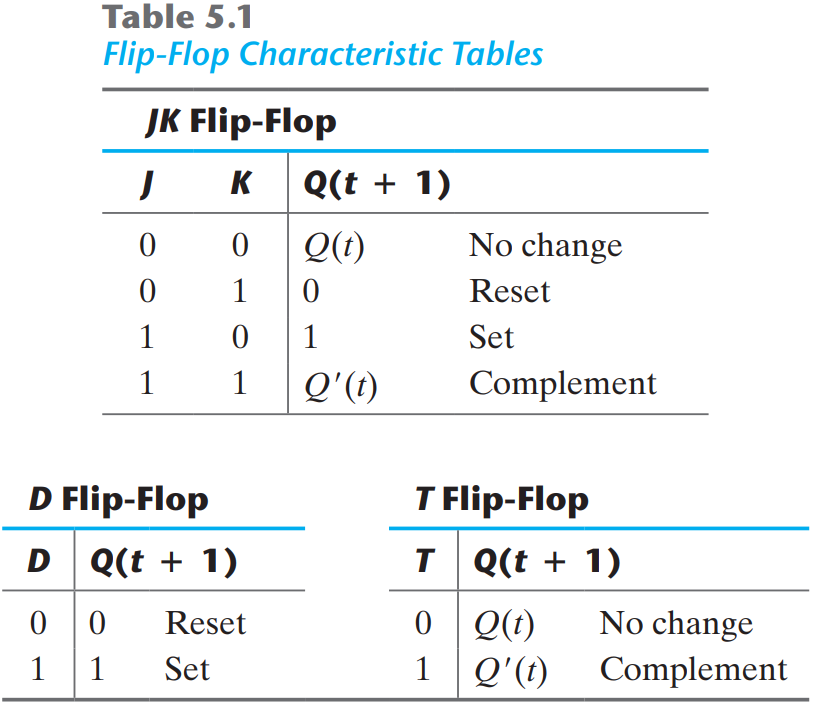
\includegraphics[width=\linewidth]{img/table-5.1.png}
  \label{table:5.1}
\end{figure}


\subsection{Characteristic Equations}
\label{subsec:char-equations}

The logical properties of a flip-flop, as described in the characteristic table, can be expressed algebraically with a characteristic equation. For the $D$ flip-flop, we have the characteristic equation
\begin{equation*}
  Q(t + 1) = D
\end{equation*}
which states that the next state of the output will be equal to the value of input $D$ in the present state. The characteristic equation for the $JK$ flip-flop can be derived from the characteristic table or from the circuit of Fig. 12. We obtain
\begin{equation*}
  Q(t + 1) = JQ' + K'Q
\end{equation*}
where $Q$ is the value of the flip-flop output prior to the application of a clock edge. The characteristic equation for the $T$ flip-flop is obtained from the circuit of Fig. 13:
\begin{equation*}
  Q(t + 1) = T \oplus Q = TQ' + T'Q
\end{equation*}


\subsection{Direct Inputs}
\label{subsec:direct-inputs}

Some flip-flops have asynchronous inputs that are used to force the flip-flop to a particular state independently of the clock. The input that sets the flip-flop to 1 is called \textit{preset} or \textit{direct set}. The input that clears the flip-flop to 0 is called \textit{clear} or \textit{direct reset}. When power is turned on in a digital system, the state of the flip-flops is unknown. The direct inputs are useful for bringing all flip-flops in the system to a known starting state prior to the clocked operation.

\begin{practice}{Practice Exercise 5.5}
Describe the functionality of a $D$-type flip-flop.

\textbf{Answer:} A $D$-type flip-flop has a $D$ (data) input, a clock input, and possibly asynchronous or synchronous clear (reset) or set signal. If \textit{set} or \textit{clear} are not asserted, the clock signal synchronizes the transfer of $D$ to $Q$, the output. If \textit{set} or \textit{reset} are asynchronous, their action controls the flip-flop independently of the clock. \textit{set} causes the output to be 1; \textit{reset} causes the output to be 0. If \textit{set} or \textit{reset} are synchronous, their action has effect at the synchronizing edge of the clock
\end{practice}

\begin{figure}[H]
  \centering
  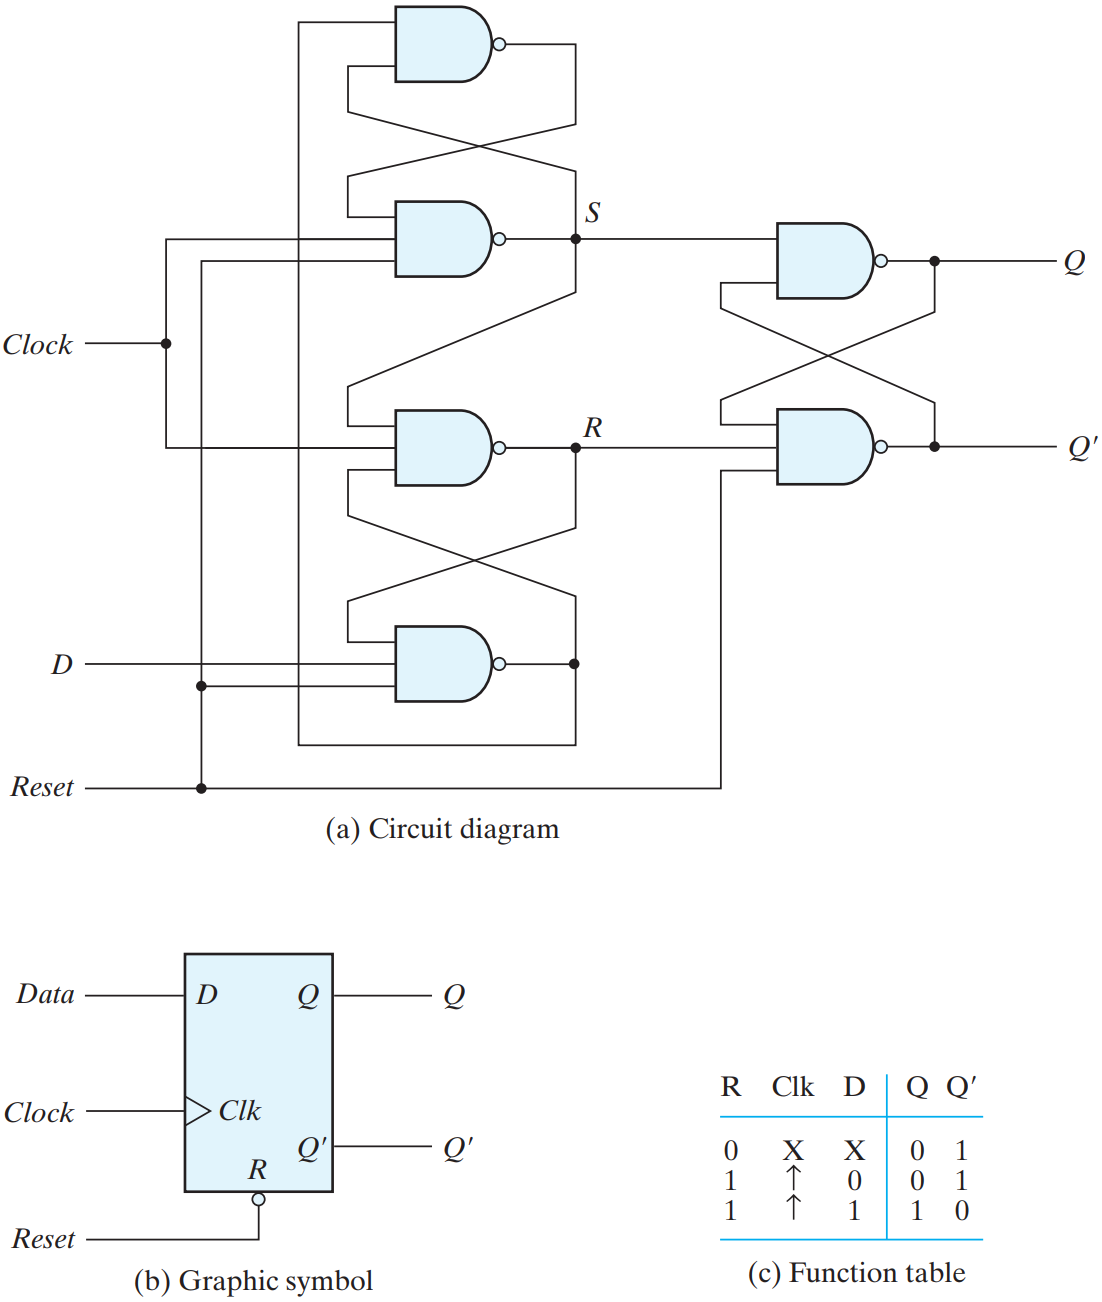
\includegraphics[width=\linewidth]{img/fig-5.14.png}
  \caption{D flip-flop with asynchronous reset}
  \label{fig:5.14}
\end{figure}

\section{Analysis of Clocked Sequential Circuits}
\label{sec:analysis-clocked-seq-circ}

Analysis describes what a given circuit will do under certain operating conditions. The behavior of a clocked sequential circuit is determined from the inputs, the outputs, and the state of its flip-flops. The outputs and the next state are both a function of the inputs and the present state.

\subsection{State Equations}
\label{subsec:state-equations}

The behavior of a clocked sequential circuit can be described algebraically by means of state equations. A \textit{state equation} (also called a \textit{transition equation}) specifies the next state as a function of the present state and inputs. Consider the sequential circuit shown in Fig. 15
\begin{figure}[H]
  \centering
  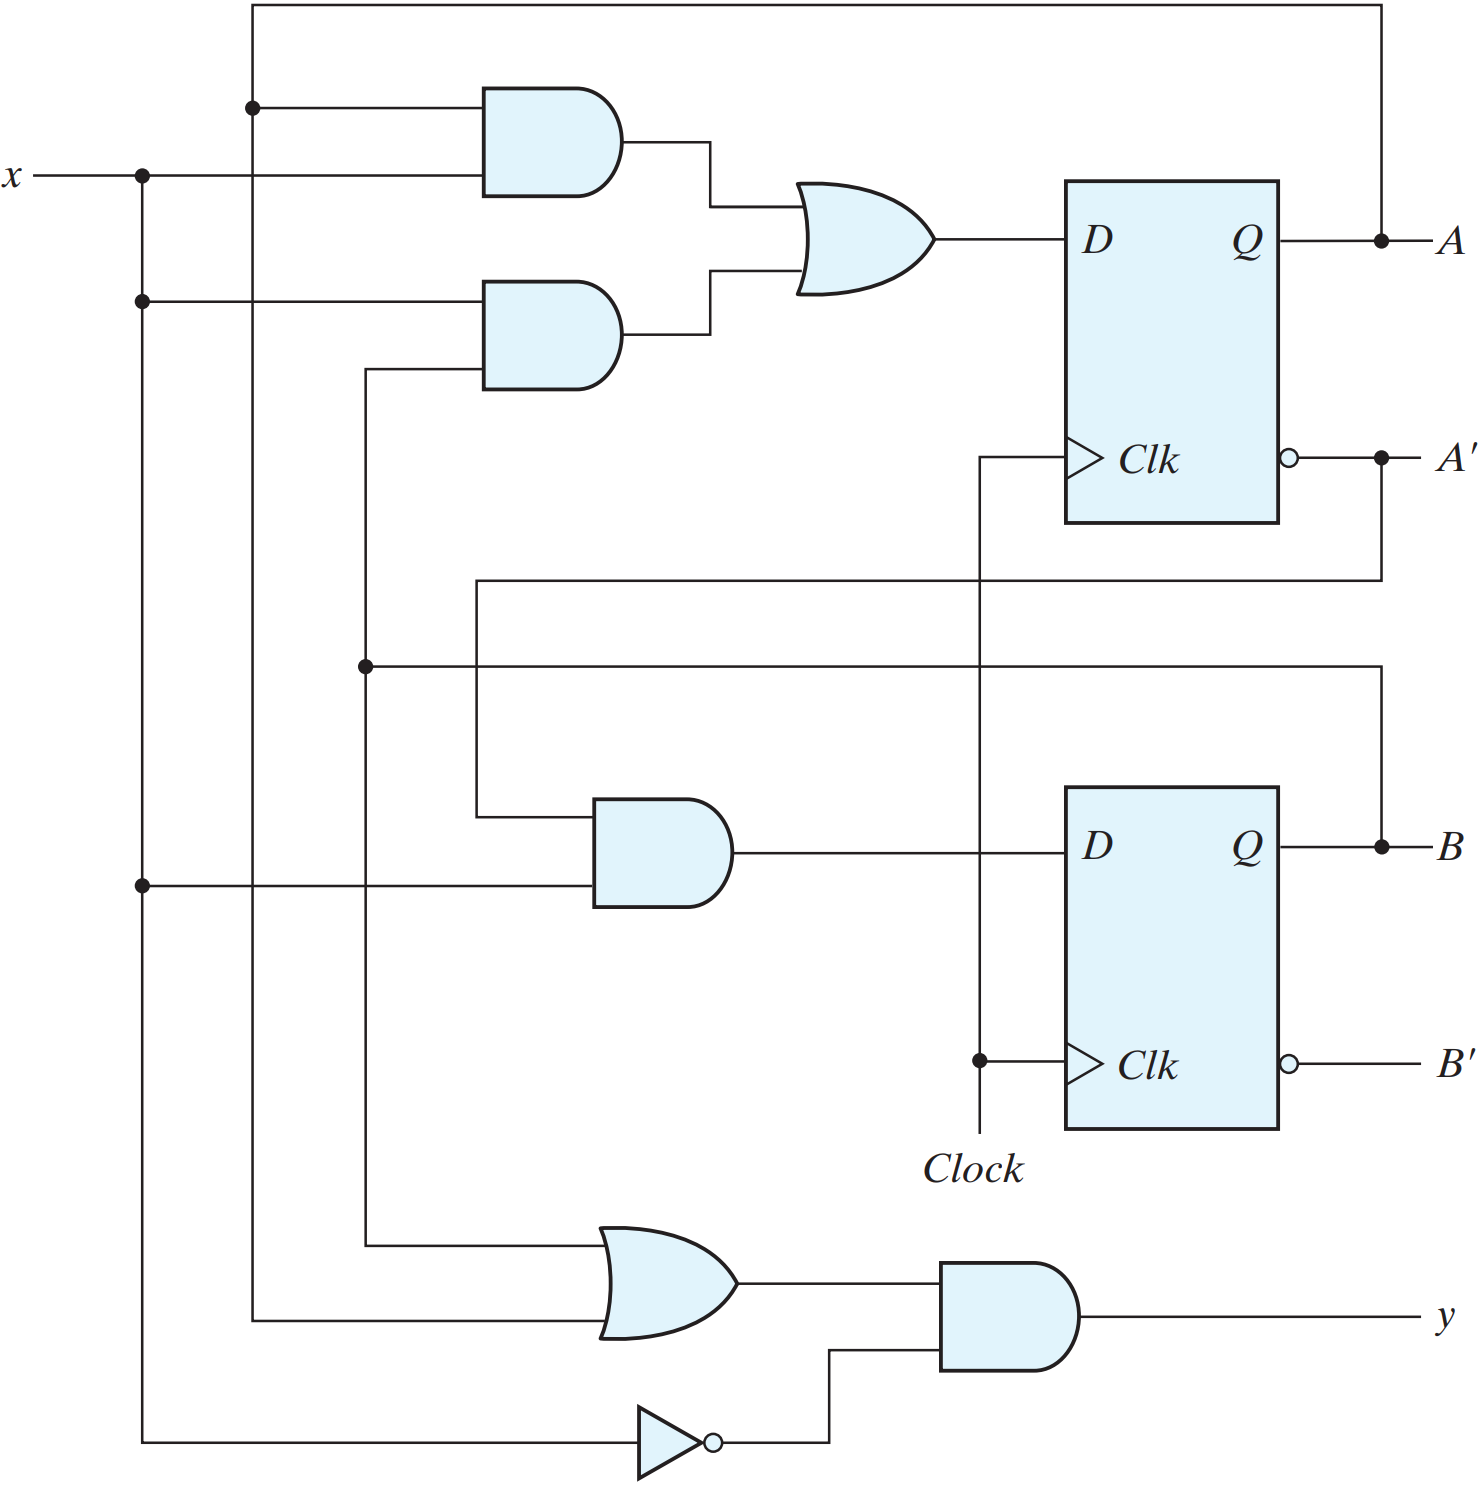
\includegraphics[width=\linewidth]{img/fig-5.15.png}
  \caption{Example of sequential circuit}
  \label{fig:5.15}
\end{figure}
It consists of two $D$ flip-flops $A$ and $B$, an input $x$ and an output $y$. Since the $D$ input of a flip-flop determines the value of the next state (i.e., the state reached after the clock transition), it is possible to write a set of state equations directly from the logic diagram in Fig. 15.
\begin{align*}
  A(t + 1) &= A(t)x(t) + B(t)x(t)\\
  B(t + 1) &= A'(t)x(t)
\end{align*}
We can omit the designation ($t$) after each variable for convenience and can express the state equations in the more compact form
\begin{align*}
  A(t + 1) &= Ax + Bx\\
  B(t + 1) &= A'x
\end{align*}
The Boolean expressions for the state equations can be derived directly from the gates that form the combinational circuit part of the sequential circuit, since the $D$ values of the combinational circuit determine the next state. Similarly, the present-state value of the output can be expressed algebraically as
\begin{equation*}
  y(t) = [A(t) + B(t)]x'(t)
\end{equation*}
By removing the symbol ($t$) for the present state, we obtain the output Boolean equation:
\begin{equation*}
  y = (A + B)x'
\end{equation*}

\subsection{State Table}
\label{subsec:state-table}

The time sequence of inputs, outputs, and flip-flop states can be enumerated in a \textit{state table} (sometimes called a \textit{transition table}). The state table for the circuit of Fig. 15 is shown in Table 5.2. The table consists of four sections labeled \textit{present state}, \textit{input}, \textit{next state}, and \textit{output}.
\begin{figure}[H]
  \centering
  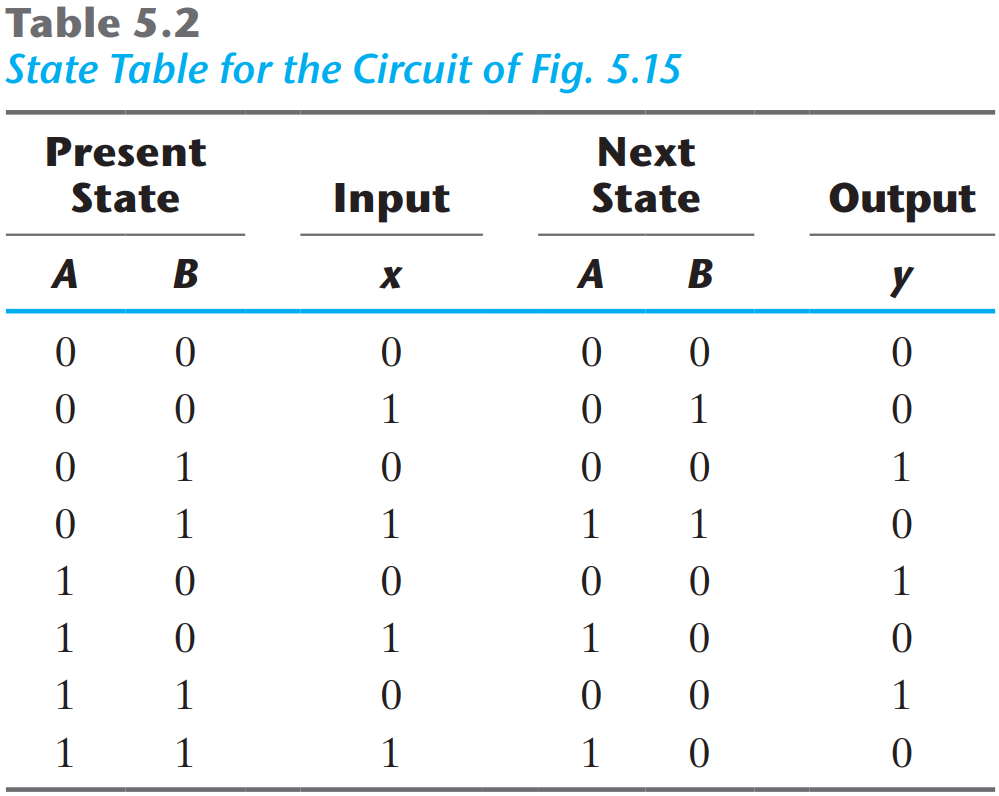
\includegraphics[width=\linewidth]{img/table-5.2.png}
  \label{table:5.2}
\end{figure}
\noindent The derivation of a state table requires listing all possible binary combinations of present states and inputs.

In general, a sequential circuit with $m$ flip-flops and $n$ inputs needs $2^{m + n}$ rows in the state table. The binary numbers from 0 through $2^{m + n - 1}$ are listed under the present state and input columns.

It is sometimes convenient to express the state table in a slightly different form having only three sections: \textit{present state}, \textit{next state}, and \textit{output}. The input conditions are enumerated under the next-state and output sections. The state table of Table 5.2 is  repeated in Table 5.3 in this second form.
\begin{figure}[H]
  \centering
  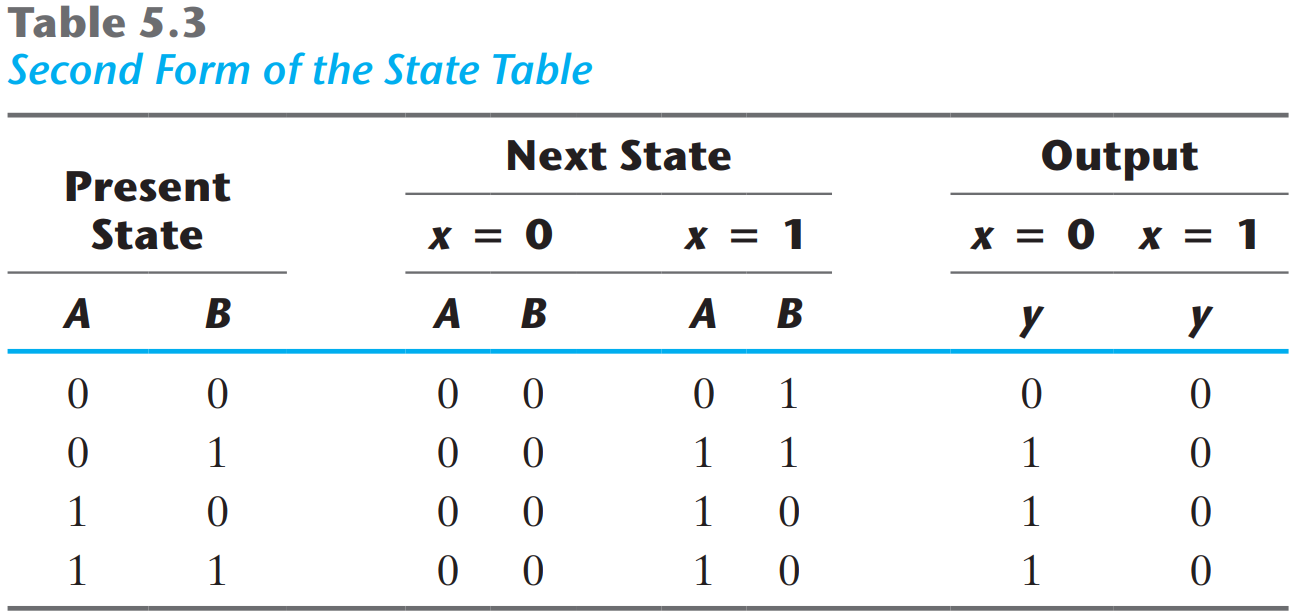
\includegraphics[width=\linewidth]{img/table-5.3.png}
  \label{table:5.3}
\end{figure}

\subsection{State Diagram}
\label{subsec:state-diagram}

The information available in a state table can be represented graphically in the form of a state diagram. In this type of diagram, a state is represented by a circle, and the (clock-triggered) transitions between states are indicated by directed lines connecting the circles.

The state diagram of the sequential circuit of Fig. 15 is shown in Fig. 16. The state diagram provides the same information as the state table and is obtained directly from Table 5.2 or Table 5.3. The binary number inside each circle identifies the state of the flip-flops. The directed lines are labeled with two binary numbers separated by a slash. The input value during the present state is labeled first, and the number after the slash gives the output during the \textit{present} state with the given input.
\begin{figure}[H]
  \centering
  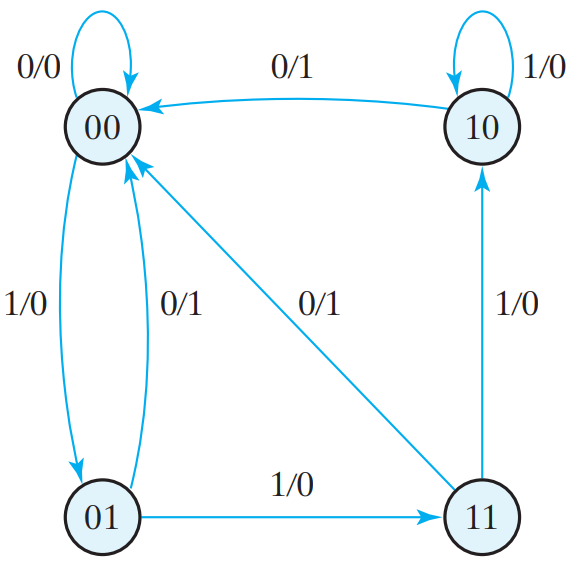
\includegraphics[width=.5\linewidth]{img/fig-5.16.png}
  \caption{State diagram of the circuit of Fig. 15}
  \label{fig:5.16}
\end{figure}

The steps presented in this example are summarized below:
\begin{center}
  Circuit diagram $\ra$ Equations $\ra$ State table $\ra$ State diagram
\end{center}

To analyze sequential circuits:
\begin{itemize}
  \item Find Boolean expressions for the outputs of the circuit and the flip-flop inputs.
  \item Use these expressions to fill in the output and flip-flop input columns in the state table.
  \item Finally, use the characteristic equation or characteristic table of the flip-flop to fill in the next state columns.
\end{itemize}
The result of sequential circuit analysis is a state table or a state diagram describing the circuit.

\textit{\textbf{Note:} There are some examples in book that are realted to analysis. Examine them carefully.}

\subsection{Mealy and Moore Models of Finite State Machine}
\label{subsec:mealy-and-moore-models}

\begin{figure}[H]
  \centering
  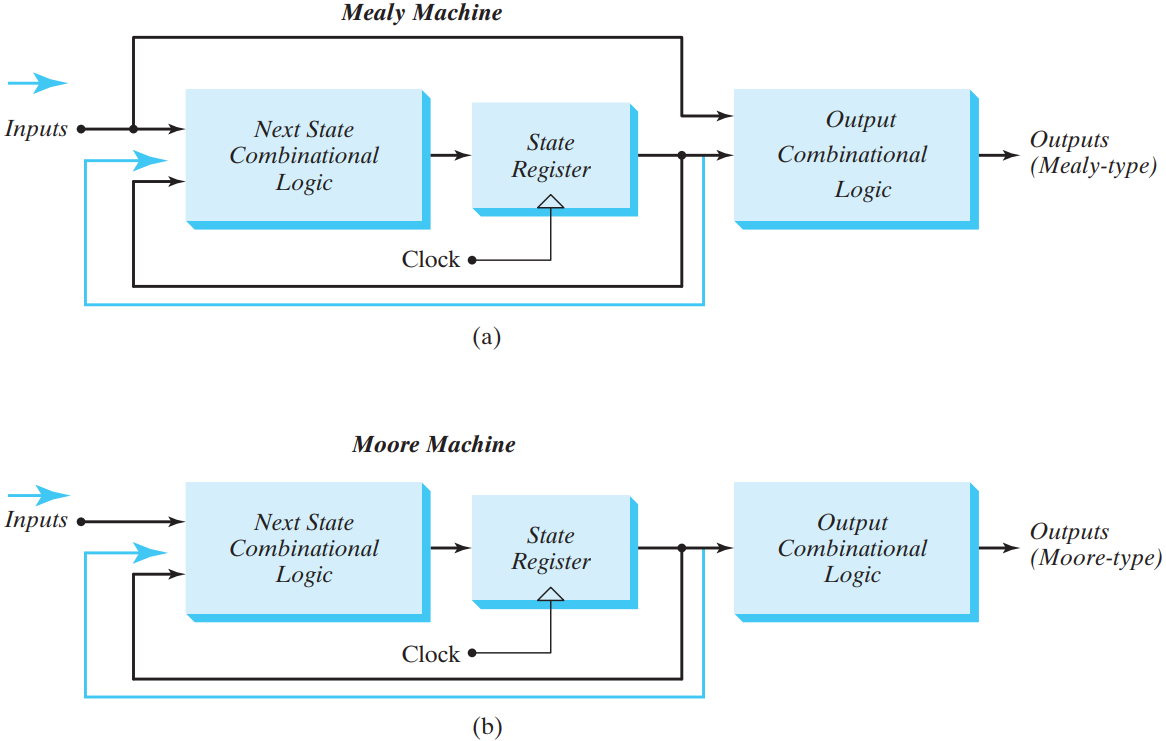
\includegraphics[width=.5\linewidth]{img/fig-5.21.png}
  \caption{}
  \label{fig:5.21}
\end{figure}

In a Moore model, the outputs of the sequential circuit are synchronized with the  clock, because they depend only on flip-flop outputs, which are synchronized with the clock.

The output of the Mealy machine is the value that is present immediately before the active edge of the clock.

\textbf{Notes:}
\begin{itemize}
  \item The difference between a Mealy and Moore state machine is that ``\textit{the output of a Moore state machine depends on only the state of the machine; the output of a Mealy machine depends on the present state and the inputs to the machine.}
  \item \textit{The edge of a state machine chart represents a transition of the machine between two states.}
  \item \textit{A transition between the states of a finite state machine occurs at the active edge of the synchronizing signal (clock).}
  \item \textit{A finite state machine may have synchronous or asynchronous reset.}
  \item The reason why it is an important practice to implement a reset  signal in a finite state machine is that ``\textit{ Without a reset signal a finite state machine cannot be driven into a known initial state.}''.
  \item \textit{The outputs of a Mealy state machine may depend on the inputs to the machine.}
\end{itemize}


\section{State Reduction and Assignment}
\label{sec:state-reduction-and-assignment}

The goal is to \textit{reduce the number of states while keeping the external input-output requirements}. $2^m$ states need $m$ flip-flops, so reducing the states may reduce flip-flops. In other words, by reducing states, number of flip-flops can also be reduced. If two states are equal, one can be removed.
\begin{quote}
  State Equivalence: ``Two states are said to be equivalent if, for each member of the set of inputs, they give exactly the same output and send the circuit either to the same state or to an equivalent state.''
\end{quote}
\noindent After a state is reduced, state table may need to be reorginazed by new state assignments.

\subsection*{Example}

As an example consider the state diagram (initially, reaching $f$ generates output 1)
\begin{figure}[H]
  \centering
  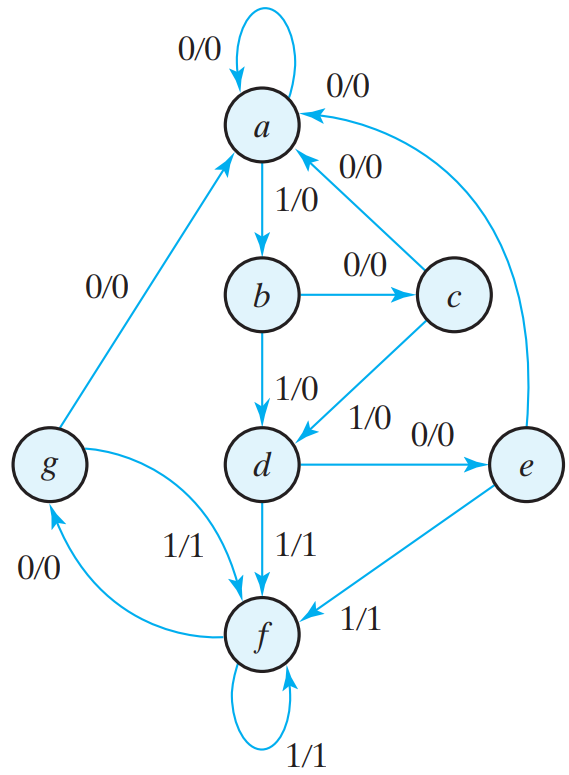
\includegraphics[width=.7\linewidth]{img/fig-5.25.png}
  \caption{A state diagram}
  \label{fig:fig5.25}
\end{figure}
The state table of the diagram is the following:
\begin{figure}[H]
  \centering
  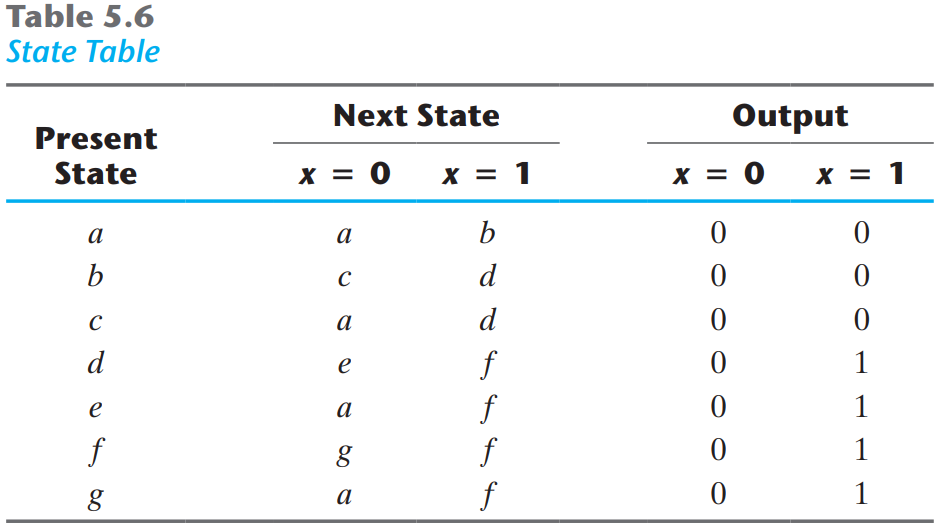
\includegraphics[width=\linewidth]{img/table-5.6.png}
  \label{table:5.6}
\end{figure}

States $e$ and $g$ are equal since for each member of the set of inputs, they give the same output and send the circuit either to the same state or an equivalent state. So one of them can be removed. So, state $g$ is removed and replaced by state $e$:
\begin{figure}[H]
  \centering
  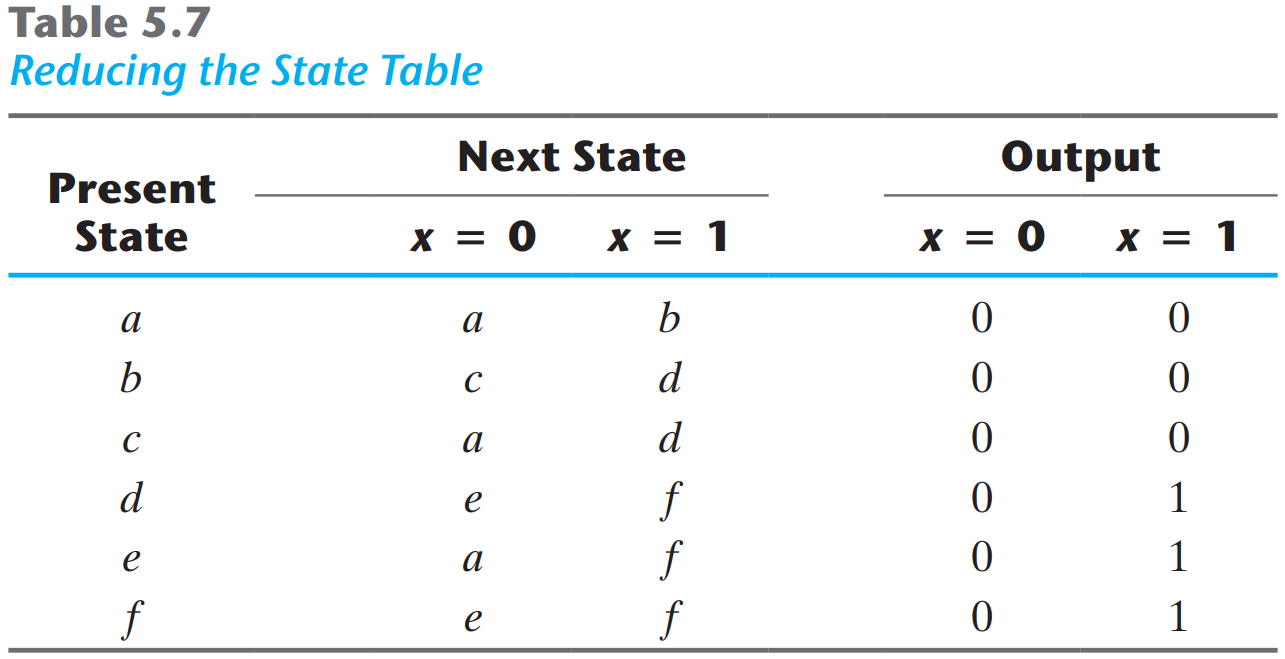
\includegraphics[width=\linewidth]{img/table-5.7.png}
  \label{table:5.7}
\end{figure}
Notice that, a state equivalence is formed. State $d$ and $f$ are equivalent. So, we can remove $f$ and replaced it with $d$:
\begin{figure}[H]
  \centering
  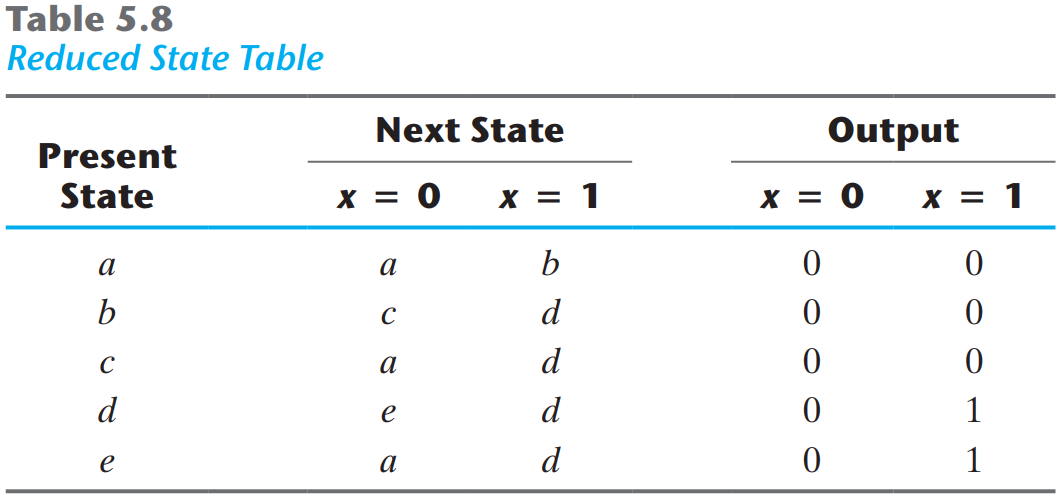
\includegraphics[width=\linewidth]{img/table-5.8.png}
  \label{table:5.8}
\end{figure}


\section{Sequential Circuit Design}
\label{sec:seq-circ-design}

Sequential circuit design is to produce a working circuit for a given description or problem.

Before starting the design procedure, there are some points to mention.

\subsection{Excitation Tables}

The flip-flop characteristic tables presented in Table 5.1 provide the value of the next state when the inputs and the present state are known. These tables are useful for analyzing sequential circuits and for defining the operation of the flip-flops. 

During the design process, we usually know the transition from the present state to the next state and wish to find the flip-flop input conditions that will cause the required transition. For this reason, we need \textit{a table that lists the required inputs for a given change of state}. Such a table is called an \textit{\textbf{excitation table}}.

\begin{figure}[H]
  \centering
  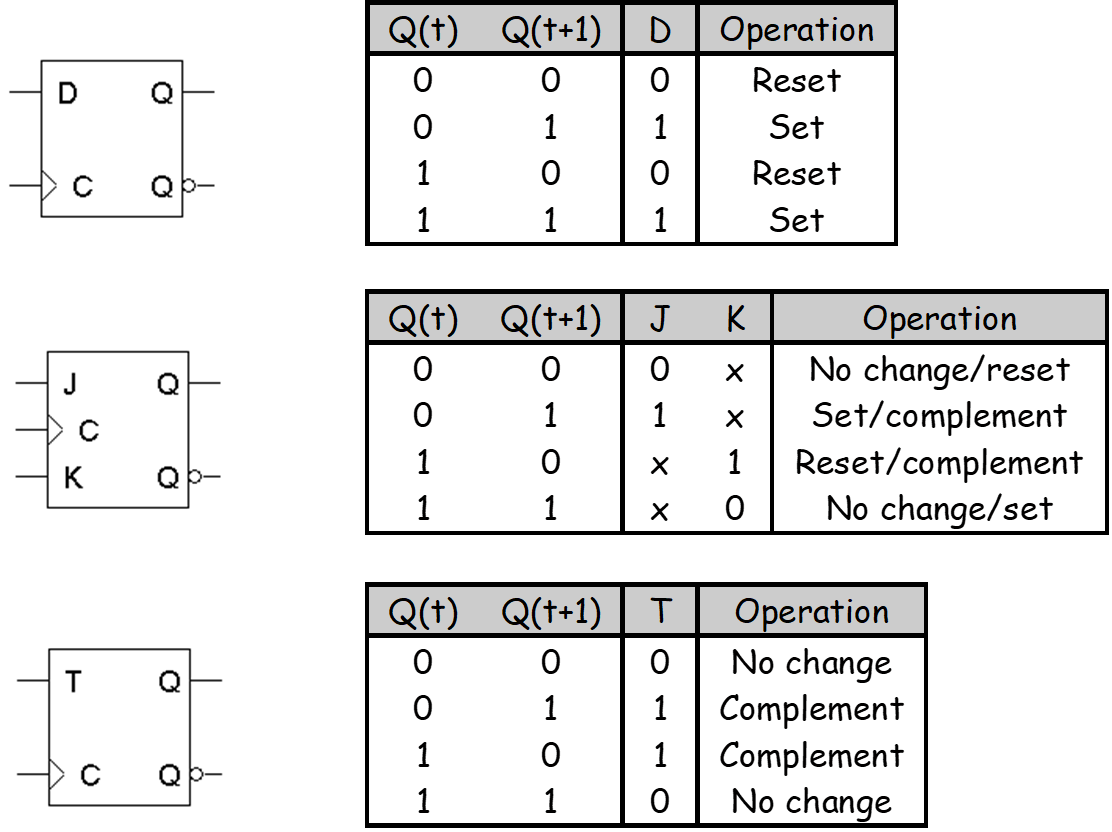
\includegraphics[width=\linewidth]{img/excitation-tables.png}
  \caption{Excitation Tables of Flip-Flops}
  \label{fig:excitation-tables}
\end{figure}

Remember the analysis steps:
\begin{itemize}
  \item Circuit diagram is given
  \item Output and next state equations
  \item State table
  \item (optional) description of what the circuit does.
\end{itemize}
Design is going through the above steps in the reverse order.

\subsection{Sequential Circuit Design Procedure}
\label{subsec:seq-circ-design-procedure}

\begin{enumerate}[label=Step\ \arabic*:, leftmargin=*]
  \item Make a state table based on the problem statement. The table should show the \textit{present states}, \textit{inputs}, \textit{next states} and \textit{outputs}. (\textit{It may be easier to find a state diagram first, and then convert that to a table.})
  \item Assign binary codes to the states in the state table (if you haven't already). If you have $n$ states, your binary codes will have at least $\lceil \log_2 n \rceil$ digits, and your circuit will have at least $\lceil \log_2 n  \rceil$ flip-flops.
  \item For each flip-flop and each row of your state table, find the flip-flop input values that are needed to generate the next state from the present state. You can use flip-flop excitation tables here.
  \item Find simplified equations for the flip-flop inputs and the outputs.
  \item Build the circuit!
\end{enumerate}

\subsection{Example: Sequence Recognizer}
\label{subsec:example-seq-recozginer}

A sequence recognizer is a special kind of sequential circuit that looks for a special bit pattern in some input. The recognizer circuit has only one input, $X$. One bit of input is supplied on every clock cycle. There is one output, $Z$, which is 1 when the desired pattern is found. 

Consider an example that the sequence recognizer will detect the bit pattern ``1001'':
\begin{align*}
  Input&:\quad 1\ 1\ 1\ 0\ 0\ 1\ 1\ 0\ 1\ 0\ 0\ 1\ 0\ 0\ 1\ 1\ 0\ \ldots\\ 
  Output&:\quad 0\ 0\ 0\ 0\ 0\ 1\ 0\ 0\ 0\ 0\ 0\ 1\ 0\ 0\ 1\ 0\ 0\ \ldots
\end{align*}
This requires a sequential circuit because the circuit has to ``remember'' the inputs from previous clock cycles, in order to determine whether or not a match was found. Here, one input and one output bit appear every clock cycle. Note that overlapping bit patterns are also detected (2nd and 3rd instances).

Remember how the state diagram arrows correspond to rows of the state table:
\begin{figure}[H]
  \centering
  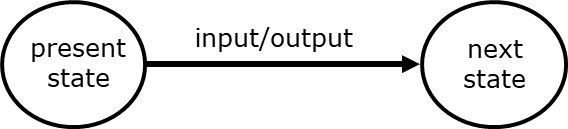
\includegraphics[width=.5\linewidth]{img/design-example-state-diagram-0.png}
\end{figure}

\subsubsection{Step 1: State Diagram (and Table)}
\label{subsubsec:step1-state-diagram-table}

What state do we need for the sequence recognizer?
\begin{itemize}
  \item We have to ``remember'' inputs from previous clock cycles.
  \item For example, if the previous three inputs were 100 and the current input is 1, then the output should be 1.
  \item In general, we will have to remember occurrences of parts of the desired pattern - in this case, 1, 10, and 100.
\end{itemize}

\begin{figure}[H]
  \centering
  \begin{minipage}{\linewidth}
    \centering
    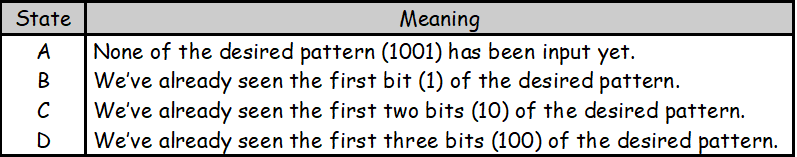
\includegraphics[width=\linewidth]{img/desing-example-table.png}
  \end{minipage}
  \begin{minipage}{\linewidth}
    \centering
    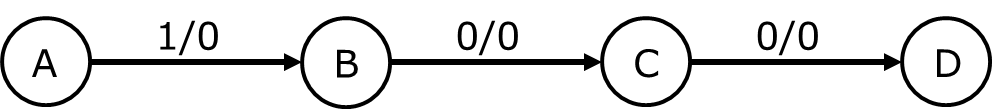
\includegraphics[width=\linewidth]{img/design-example-state-diagram.png}
  \end{minipage}
\end{figure}

What happens if we're in state D (the last three inputs were 100), and the current input is 1?
\begin{itemize}
  \item The output should be a 1, because we've found the desired pattern.
  \item But this last 1 could also be the start of another occurrence of the pattern! For example, 1001001 contains two occurrences of 1001.
  \item To detect overlapping occurrences of the pattern, the next state should be B.
\end{itemize}
\begin{figure}[H]
  \centering
  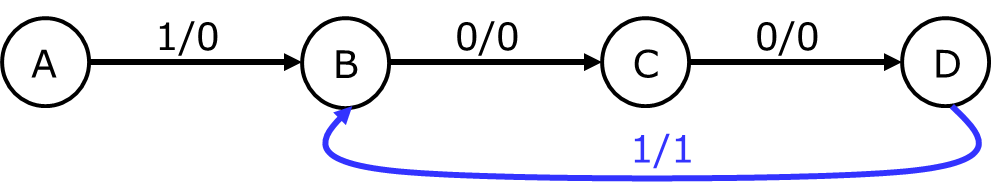
\includegraphics[width=.85\linewidth]{img/design-example-state-diagram-2.png}
\end{figure}

Remember that we need two outgoing arrows for each node, to account for the possibilities of $X = 0$ and $X = 1$. They also allow for the correct detection of overlapping occurrences of 1001.
\begin{figure}[H]
  \centering
  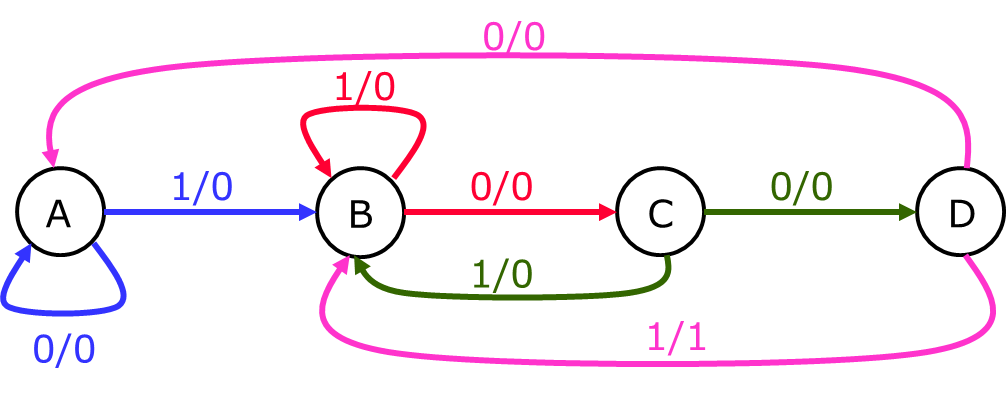
\includegraphics[width=\linewidth]{img/design-example-state-diagram-4.png}
\end{figure}
\noindent Finally, making the state table.
\begin{figure}[H]
  \centering
  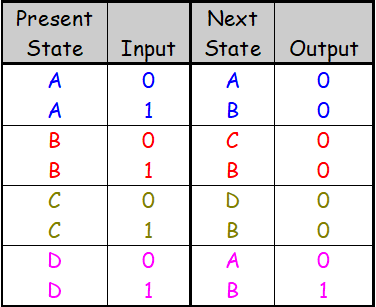
\includegraphics[width=.8\linewidth]{img/desing-example-state-table.png}
\end{figure}

\subsubsection{Step 2: Assigning Binary Codes}
\label{subsubsec:step2-assign-bin-code}

We have four states ABCD, so we need at least two flip-flops $Q_1Q_0$. The easiest thing to do is represent state A with $Q_1Q_0 = 00$, B with 01, C with 10, and D with 11 (intuitive).
\begin{figure}[H]
  \centering
  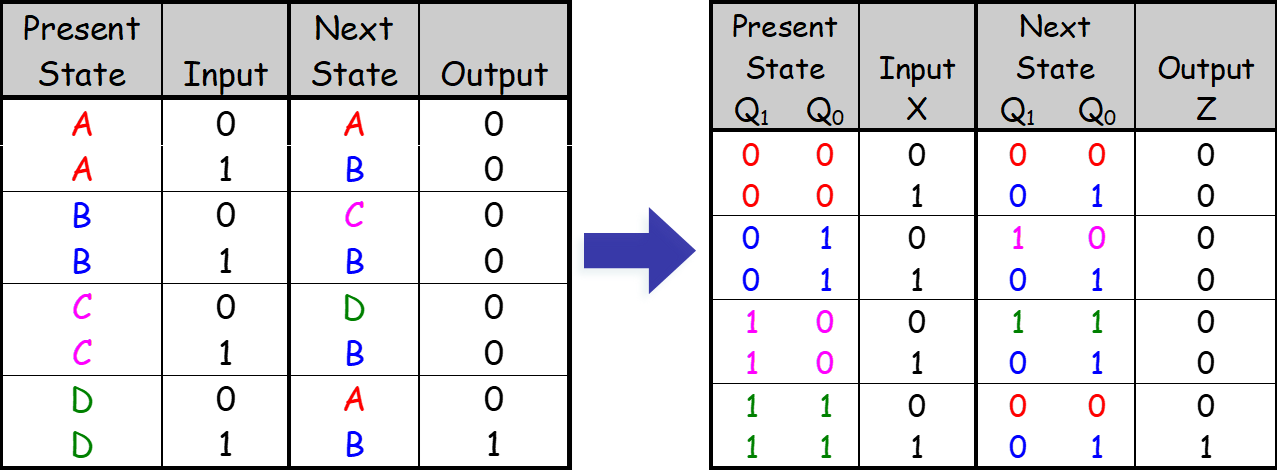
\includegraphics[width=\linewidth]{img/desing-example-state-table-2.png}
\end{figure}

\subsubsection{Step 3: Finding Flip-Flop Inputs}
\label{subsubsec:step3-finding-ff-inputs}

Next we have to figure out how to actually make the flip-flops change from their present state into the desired next state. This depends on what kind of flip-flops you use! We'll use two $JK$s. For each flip-flip $Q_i$, look at its present and next states, and determine what the inputs $J_i$ and $K_i$ should be in order to make that state change.

While doing this, we can use excitation table of $JK$ flip-flop. For example, if the present state of a JK flip-flop is 0 and we want the next state to be 1, then we have two choices for the JK inputs: $JK = 10$ or $JK = 11$.
\begin{figure}[H]
  \centering
  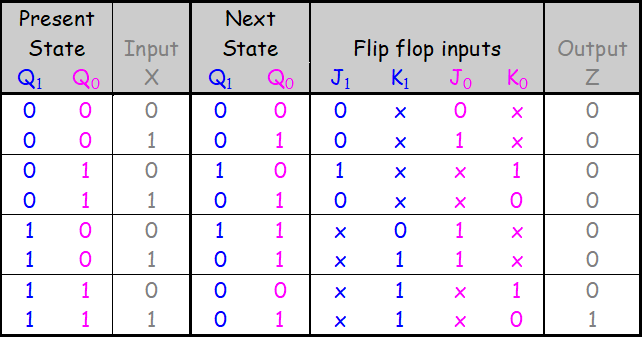
\includegraphics[width=\linewidth]{img/desing-example-state-table-3.png}
\end{figure}

\subsubsection{Step 4: Find Flip-Flop In/Out Equations}
\label{subsubsec:step4-find-ff-io-equations}

Now one can make K-maps and find equations for each of the four flip-flop inputs, as well as for the output $Z$. These equations are in terms of the present state and the inputs. The advantage of using $JK$ flip-flops is that there are many don't care conditions, which can result in simpler equations. In the end, the following equations can be found:
\begin{align*}
	J_0 &= X + Q_1\\
	K_0 &= X'\\
  &\\
  J_1 &= X'Q_0\\
	K_1 &= X + Q0\\
  &\\
	Z &= Q_1Q_0X
\end{align*}

\subsubsection{Step 5: Build the Circuit}
\label{subsubsec:step5-build-the-circuit}

Lastly, we use these simplified equations to build the completed circuit.
\begin{figure}[H]
  \centering
  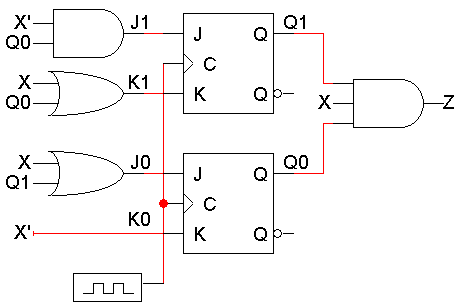
\includegraphics[width=\linewidth]{img/design-example-circuit.png}
\end{figure}


\end{multicols*}

\end{document}
